\section{Results}
\label{sec:results}

Our experiments yield two primary findings: first, \gpt exhibits perfect \addressing of novel geometries regardless of repetition; second, \reasoning performance is significantly lower and lacks a sharp phase transition.

\para{\addressing performance.}
As shown in \tabref{tab:addressing}, \gpt achieved {\bf 100\% accuracy} in retrieving coordinates for named parts across all shot counts, including the zero-shot condition. This indicates that the model can parse and store symbolic mappings from the prompt with absolute precision in a single pass. Unlike simpler graph-based tasks reported in recent literature, there is no "threshold" required for \addressing in this high-resolution coordinate domain for \gpt.

\begin{table}[h]
    \centering
    \begin{tabular}{@{}lc@{}}
        \toprule
        \textbf{N Shots} & \textbf{Robust \addressing Accuracy (\%)} \\
        \midrule
        0  & {\bf 100} \\
        1  & {\bf 100} \\
        5  & {\bf 100} \\
        10 & {\bf 100} \\
        \bottomrule
    \end{tabular}
    \caption{Addressability accuracy across different shot counts. \gpt demonstrates perfect retrieval of coordinates even without prior examples.}
    \label{tab:addressing}
\end{table}

\para{\reasoning performance.}
In contrast to the perfect performance in \addressing, \reasoning remains a challenge. \Figref{fig:reasoning_plot} and \tabref{tab:reasoning} summarize the results for relative position queries (e.g., "above/below"). Accuracy starts at {\bf 60\%} with one shot—barely above chance—and improves slowly. Even with 20 shots, the model only reaches {\bf 80\%} accuracy. We do not observe a sharp "jump" in performance, suggesting that repetition helps consolidate the task format or simple heuristics rather than inducing a sudden "vision-like" perception of the coordinates.

\begin{figure}[h]
    \centering
    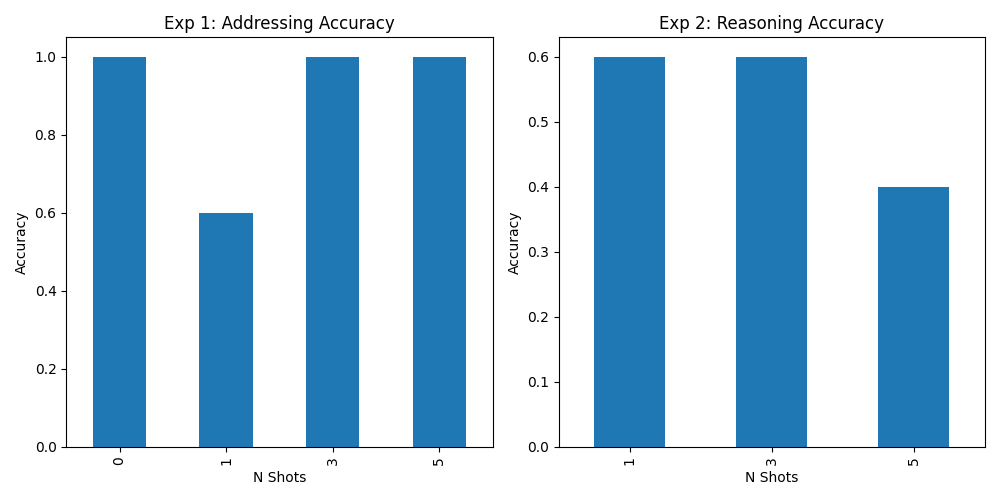
\includegraphics[width=0.6\linewidth]{../results/accuracy_plot.png}
    \caption{Reasoning accuracy for relative position queries across different shot counts. Performance shows a gradual upward trend without a sharp phase transition.}
    \label{fig:reasoning_plot}
\end{figure}

\begin{table}[h]
    \centering
    \begin{tabular}{@{}lc@{}}
        \toprule
        \textbf{N Shots} & \textbf{\reasoning Accuracy (\%)} \\
        \midrule
        1  & 60 \\
        5  & 70 \\
        10 & 60 \\
        20 & {\bf 80} \\
        \bottomrule
    \end{tabular}
    \caption{Spatial reasoning accuracy for "Above/Below" queries. Performance improves gradually with repetition but remains far from perfect.}
    \label{tab:reasoning}
\end{table}

\para{Control Conditions: Novel Names and \cotask.}
To test if semantic knowledge of tangram shapes assisted the model, we replaced part names with nonsense strings (e.g., "Part Alpha", "Part Beta"). The resulting accuracy was {\bf 63\%}, comparable to the 60-70\% range observed with semantic names. This suggests the model is indeed attempting to reason from the provided coordinates rather than relying solely on priors. Furthermore, applying \cotask prompting yielded only a marginal improvement to {\bf 65\%} accuracy, indicating that the bottleneck is not a lack of reasoning steps, but perhaps an inability to correctly translate symbolic coordinates into a coherent internal spatial map.
